A primeira abordagem para realizar a montagem experimental foi construir uma placa de circuito impresso com o circuito do Mazzilli. Porém, o circuito planejado drenaria uma corente de 30A e oscilaria numa frequência em torno de 400kHz. Utilizando [] para calcular qual deveria ser o tamanho da trilha, chegamos a valores que não seriam práticos. Portanto a ideia era fazer a montagem em outro material e fazer as ligações por cabos que se usam em instalação elétrica, garantindo assim o funcionamento adequado. Para isto, foi feita a montagem experimental em cima de uma placa de madeira, que é um péssimo condutor, funcionando como um ótimo isolante. 
\section{Transistores}
Para podermos atender os requisitos citados em [] foi necessário a escolha de um IRFP250N, onde podemos conferir suas especificações [] na tabela X.
\section{Capacitores}
Outro problema prático é que o capacitor deve ser apolar, pois o sinal excursionado nele ora é positivo, ora é negativo. Além disto, a corrente AC que passa está na ordem de XXA, havendo a necessidade de realizar associações em paralelo para dividir a corrente entre os componentes até um valor aceitável. A \ref{tabela-cap-comp} mostra os materiais que são comumente fabricados o capacitor. Podemos observar que o melhor material para agir em conjunto com um circuito que irá oscilar em 400khz, com uma alta tensão e maior fator de qualidade possível, é o polipropilêno. No projeto, foi utilizado 3 capacitores, modelo XXXX [].


\begin{table}[htb]
\IBGEtab{%
  \caption{Comparativo entre os tipos de capacitores.}%
  \label{tabela-cap-comp}
}{%
  \begin{tabular}{cccccc}
  \toprule
  Tipo & Polaridade & Potência & Escala & ESR & Frequência de Operação \\
  \midrule
  Cerâmica & Não & Baixa & $\mu F$ & Baixo & Alta \\
  Poliestireno & Não & Alta & $pF$ & Baixo & Muito Alta \\
  Poliester & Não	& Alta & $\mu F$ & Baixo & Muito Alta \\
  Polipropilêno & Não & Alta & $\mu F$ & Muito baixo & Muito Alta \\
  Eletrolítico & Não* & Alta & $F$ & Alta & Baixa \\
  \bottomrule
\end{tabular}%
}{%
  \fonte{Wikipédia}%
  \nota{\hyphenation{Equivalent Series Resistence }: uma medida de não idealidade do componente que mede o valor da resistência em série com o mesmo para uma determinada frequência.}%
  \nota[Anotações]{* Existem os capacitores eletrolíticos bipolares porém não possuem capacitâncias tão altas.}%
  }
\end{table}



\section{Bobina de Trabalho}

\section{Choke}
Utilizando a fórmula aproximada de Wheeler [], adaptado em [], para ficar em metros e Henrys, temos que a fórmula explicita para o cálculo da indutância é:
\begin{equation}
L = \mu_0 \frac{\pi r^2 n^2}{h + 0.9r}
\end{equation}
Onde $ L$ é a indutância desejada, $\mu_0$ é a permeabilidade no ar, $r$ o raio da seção de reta do indutor, $n$ o número de espiras e $h$ a altura da bobina. Variando os parâmetros $r$, $h$ e $L$, considerando $h = 3r$ temos a tabela X.
Com isso temos um valor de N espiras, não sendo viável produzir artesanalmente o choke. Para sanar o problema, recorremos ao uso de chokes em fontes chaveadas de computadores, onde possuem as mesmas características requerida pelo projeto. Essas fontes normalmente para gabinete ATX, possuem um choke com núcleo de ferrite (ve \ref{fig_fonte-atx}), reduzindo o número de espiras drasticamente.

\begin{figure}[htb]
\caption{\label{fig_fonte-atx}Demonstração do choke na fonte ATX}
\begin{center}
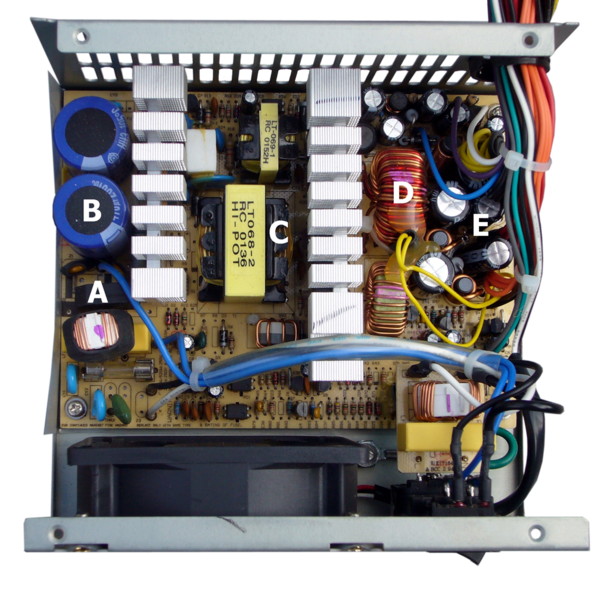
\includegraphics[scale=0.5]{images/fonte-atx.png}
\end{center}
\legend{Observe o choke, marcado com a letra 'D', de uma fonte ATX com núcleo de ferrite enrolado com várias espiras. Fonte: Wikipedia.}
\end{figure}


\section{Diodo de recuperação rápida}
O diodo que realiza o chaveamento do transistor no momento certo, ajudando a descarregar a base, deve poder responder na mesma velocidade de chaveamento necessária no circuito, com isso utilizamos o diodo XXXXX, com resposta de XXXX.
\section{Fonte}
Um dos fatores cruciais do projeto é a fonte de alimentação. Ela deve ser capaz de fornecer uma energia de NNNW, uma corrente de XXXXA e ideal seria uma tensão regulada. No entanto, como o projeto em si é uma prova de conceito, não foi possível conseguir uma fonte de tensão regulável. Por fim, utilizamos uma bateria de chumbo, modelo XXXX, de XXXXXXAh. (ver foto)
\section{Montagem}
Utilizamos solda de estanho e fios de $XXmmm^2$ e $XXmm^2$ para a parte de baixa e alta tensão, respectivamente. A montagem final pode ser conferida na figura XX.